% Generated by code/needham.py -- do not edit by hand.
\definecolor{qocA}{rgb}{0.00,0.45,0.70}
\definecolor{qocB}{rgb}{0.90,0.60,0.00}
\definecolor{qocC}{rgb}{0.00,0.62,0.45}
\definecolor{qocD}{rgb}{0.80,0.40,0.00}
\definecolor{qocE}{rgb}{0.80,0.60,0.70}
\definecolor{qocF}{rgb}{0.35,0.70,0.90}
\begin{tikzpicture}[ink/.style={line width=0.9pt, ndInk}, faint/.style={line width=0.4pt, ndInk!35}, dashedink/.style={line width=0.5pt, ndInk!55, dash pattern=on 2.5pt off 2pt}, vec/.style={->, >=stealth, line width=1.2pt}, note/.style={font=\footnotesize\itshape, text=ndInk!85, align=center}, pointer/.style={->, >=stealth, line width=0.4pt, ndInk!60, shorten >=2pt, shorten <=1pt}, dot/.style={circle, fill=ndInk, inner sep=0pt, minimum size=3.4pt}, wash/.style={fill=ndSky, fill opacity=0.55}, every node/.style={text=ndInk}]
\definecolor{ndInk}{rgb}{0.13,0.13,0.18}
\definecolor{ndPaper}{rgb}{0.99,0.96,0.88}
\definecolor{ndSky}{rgb}{0.84,0.91,0.98}
\definecolor{ndRose}{rgb}{0.98,0.86,0.84}
\definecolor{ndBlue}{rgb}{0.13,0.36,0.66}
\definecolor{ndRed}{rgb}{0.78,0.20,0.16}
\definecolor{ndGold}{rgb}{0.88,0.62,0.10}
\definecolor{ndGreen}{rgb}{0.18,0.52,0.30}
\node[font=\tiny, text=ndInk!60] at (1.550,4.550) {1};
\node[font=\tiny, text=ndInk!60] at (2.070,4.550) {2};
\node[font=\tiny, text=ndInk!60] at (2.590,4.550) {3};
\node[font=\tiny, text=ndInk!60] at (5.350,4.550) {1};
\node[font=\tiny, text=ndInk!60] at (5.870,4.550) {2};
\node[font=\tiny, text=ndInk!60] at (6.390,4.550) {3};
\node[font=\scriptsize, text=ndInk!70] at (0.800,4.550) {qubit};
\draw[line width=7pt, ndGreen!35, line cap=round] (1.550,4.050) -- (1.551,4.050);
\draw[ink, fill=ndGreen!25] (1.550,4.050) circle (0.190);
\node[font=\scriptsize] at (1.550,4.050) {$Z$};
\draw[faint, fill=white] (2.070,4.050) circle (0.190);
\node[font=\scriptsize, text=ndInk!40] at (2.070,4.050) {$I$};
\draw[faint, fill=white] (2.590,4.050) circle (0.190);
\node[font=\scriptsize, text=ndInk!40] at (2.590,4.050) {$I$};
\node[font=\scriptsize, anchor=east] at (1.250,4.050) {$-\imath Z_1$};
\draw[line width=7pt, ndBlue!35, line cap=round] (1.550,3.400) -- (2.071,3.400);
\draw[ink, fill=ndBlue!25] (1.550,3.400) circle (0.190);
\node[font=\scriptsize] at (1.550,3.400) {$X$};
\draw[ink, fill=ndBlue!25] (2.070,3.400) circle (0.190);
\node[font=\scriptsize] at (2.070,3.400) {$X$};
\draw[faint, fill=white] (2.590,3.400) circle (0.190);
\node[font=\scriptsize, text=ndInk!40] at (2.590,3.400) {$I$};
\node[font=\scriptsize, anchor=east] at (1.250,3.400) {$-\imath X_1X_2$};
\draw[ink] (1.300,3.000) -- (2.840,3.000);
\draw[line width=7pt, ndBlue!35, line cap=round] (1.550,2.550) -- (2.071,2.550);
\draw[ink, fill=ndBlue!25] (1.550,2.550) circle (0.190);
\node[font=\scriptsize] at (1.550,2.550) {$Y$};
\draw[ink, fill=ndBlue!25] (2.070,2.550) circle (0.190);
\node[font=\scriptsize] at (2.070,2.550) {$X$};
\draw[faint, fill=white] (2.590,2.550) circle (0.190);
\node[font=\scriptsize, text=ndInk!40] at (2.590,2.550) {$I$};
\node[font=\scriptsize, anchor=east] at (1.250,2.550) {$\tfrac12[\,\cdot\,,\cdot\,]$};
\node[note, anchor=north] at (2.070,2.150) {a 1-local string with a\\ 2-local one: the bracket\\ stays inside the support};
\draw[line width=7pt, ndBlue!35, line cap=round] (5.350,4.050) -- (5.871,4.050);
\draw[ink, fill=ndBlue!25] (5.350,4.050) circle (0.190);
\node[font=\scriptsize] at (5.350,4.050) {$Z$};
\draw[ink, fill=ndBlue!25] (5.870,4.050) circle (0.190);
\node[font=\scriptsize] at (5.870,4.050) {$Z$};
\draw[faint, fill=white] (6.390,4.050) circle (0.190);
\node[font=\scriptsize, text=ndInk!40] at (6.390,4.050) {$I$};
\node[font=\scriptsize, anchor=east] at (5.050,4.050) {$-\imath Z_1Z_2$};
\draw[line width=7pt, ndBlue!35, line cap=round] (5.870,3.400) -- (6.391,3.400);
\draw[faint, fill=white] (5.350,3.400) circle (0.190);
\node[font=\scriptsize, text=ndInk!40] at (5.350,3.400) {$I$};
\draw[ink, fill=ndBlue!25] (5.870,3.400) circle (0.190);
\node[font=\scriptsize] at (5.870,3.400) {$X$};
\draw[ink, fill=ndBlue!25] (6.390,3.400) circle (0.190);
\node[font=\scriptsize] at (6.390,3.400) {$X$};
\node[font=\scriptsize, anchor=east] at (5.050,3.400) {$-\imath X_2X_3$};
\draw[ink] (5.100,3.000) -- (6.640,3.000);
\draw[line width=7pt, ndRed!35, line cap=round] (5.350,2.550) -- (6.391,2.550);
\draw[ink, fill=ndRed!25] (5.350,2.550) circle (0.190);
\node[font=\scriptsize] at (5.350,2.550) {$Z$};
\draw[ink, fill=ndRed!25] (5.870,2.550) circle (0.190);
\node[font=\scriptsize] at (5.870,2.550) {$Y$};
\draw[ink, fill=ndRed!25] (6.390,2.550) circle (0.190);
\node[font=\scriptsize] at (6.390,2.550) {$X$};
\node[font=\scriptsize, anchor=east] at (5.050,2.550) {$\tfrac12[\,\cdot\,,\cdot\,]$};
\node[note, anchor=north, text=ndRed] at (5.870,2.150) {two 2-local strings\\ sharing a qubit: the\\ bracket is 3-local};
\node[font=\small, anchor=north] at (3.750,0.550) {(a) supports and brackets};
\draw[faint, ->, >=stealth] (8.700,1.000) -- (11.404,1.000) node[right, text=ndInk] {};
\draw[faint, ->, >=stealth] (8.700,1.000) -- (8.700,4.816) node[above, text=ndInk] {{\scriptsize dimension}};
\draw[faint] (8.760,2.851) -- (8.640,2.851) node[left, font=\scriptsize, text=ndInk] {$36$};
\draw[faint] (8.760,4.240) -- (8.640,4.240) node[left, font=\scriptsize, text=ndInk] {$63$};
\filldraw[fill=ndGreen!35, draw=ndGreen!70!ndInk, line width=0.4pt] (9.055,1.000) rectangle (9.764,1.463);
\filldraw[fill=ndBlue!35, draw=ndBlue!70!ndInk, line width=0.4pt] (9.055,1.463) rectangle (9.764,2.851);
\node[font=\scriptsize, anchor=north] at (9.409,0.923) {$\mathfrak d$};
\filldraw[fill=ndGreen!35, draw=ndGreen!70!ndInk, line width=0.4pt] (10.236,1.000) rectangle (10.945,1.463);
\filldraw[fill=ndBlue!35, draw=ndBlue!70!ndInk, line width=0.4pt] (10.236,1.463) rectangle (10.945,2.851);
\filldraw[fill=ndRed!35, draw=ndRed!70!ndInk, line width=0.4pt] (10.236,2.851) rectangle (10.945,4.240);
\node[font=\scriptsize, anchor=north] at (10.591,0.923) {$\mathfrak d+[\mathfrak d,\mathfrak d]$};
\draw[dashedink] (8.700,4.240) -- (11.300,4.240) node[right, font=\scriptsize, text=ndInk] {$\liesu[8]$};
\node[font=\tiny, text=ndGreen!70!ndInk] at (10.591,1.231) {1-qubit, 9};
\node[font=\tiny, text=ndBlue!70!ndInk] at (10.591,2.157) {2-qubit, 27};
\node[font=\tiny, text=ndRed!70!ndInk] at (10.591,3.546) {3-qubit, 27};
\node[font=\small, anchor=north] at (10.000,0.383) {(b) one bracket fills $\liesu[8]$};
\draw[faint, ->, >=stealth] (12.750,1.000) -- (16.286,1.000) node[right, text=ndInk] {};
\draw[faint, ->, >=stealth] (12.750,1.000) -- (12.750,4.816) node[above, text=ndInk] {{\scriptsize 3-qubit directions reached}};
\draw[faint] (12.810,2.440) -- (12.690,2.440) node[left, font=\scriptsize, text=ndInk] {$12$};
\draw[faint] (12.810,3.880) -- (12.690,3.880) node[left, font=\scriptsize, text=ndInk] {$24$};
\draw[faint] (12.810,4.240) -- (12.690,4.240) node[left, font=\scriptsize, text=ndInk] {};
\draw[dashedink] (12.750,4.240) -- (16.150,4.240) node[right, font=\scriptsize, text=ndInk] {$27$};
\draw[line width=1.2pt, ndGreen] (12.987,1.018) -- (13.646,1.018);
\node[font=\scriptsize, anchor=south, text=ndGreen!70!ndInk] at (13.317,1.072) {$0$};
\node[font=\scriptsize, anchor=north] at (13.317,0.820) {1-local};
\filldraw[fill=ndRed!35, draw=ndRed!70!ndInk, line width=0.4pt] (14.120,1.000) rectangle (14.780,2.440);
\node[font=\scriptsize, anchor=north] at (14.450,0.820) {$Z_1Z_2$};
\filldraw[fill=ndRed!35, draw=ndRed!70!ndInk, line width=0.4pt] (15.254,1.000) rectangle (15.913,3.880);
\node[font=\scriptsize, anchor=north] at (15.583,0.820) {2-local};
\node[note, anchor=north] at (14.450,0.340) {drift $H_d$; bars: rank of\\ $[-\imath H_d,\mathfrak d]$ outside $\mathfrak d$};
\node[font=\small, anchor=north] at (14.450,-0.440) {(c) which drifts normalise $\mathfrak d$};
\end{tikzpicture}
